\section{Abstract Interpretation}

Abstract interpretation \cite{Cousot77, Cousot21} is the de-facto standard
approach for designing static program analysis. The specification of a program
can be expressed as a pair of initial and final sets of states, $Init, Final
\in \pow{\states}$, and the task of verifying a program $C$ boils down to
checking if $\sem{C}(Init) \subseteq Final$.

Clearly, this task cannot be performed in general. The solution proposed by the
framework of abstract interpretation is to construct an approximation of
$\sem{\cdot}$, usually denoted by $\sem{\cdot}^\#$, that is computable.

\subsection{Abstract Domains}

One of the techniques used by abstract interpretation to make the problem of 
verification tractable involves representing collections of states with a finite 
amount of memory.

\begin{definition}[Abstract Domain]
  A poset $(A, \leq)$ is an abstract domain if there exists a Galois insertion
  $\langle \pow{\states}, \subseteq \rangle \galoiS{\alpha}{\gamma} \langle A, 
  \leq \rangle$.
\end{definition}

\begin{example}[Interval Domain]
  \label{exmp:interval}
  Let $Int = \{ [a, b] \mid a, b \in \mathbb{Z} \cup \{+\infty, -\infty \}, a 
  \leq b \} \cup \{ \bot \}$ be ordered by inclusion, each element $[a, b]$ 
  represent the set $\{ x \mid a \leq x \leq b \}$ and $\bot$ is used as a 
  representation of $\emptyset$. The structure of the 
  lattice can be summarized by the following Hasse diagram:

  \begin{center}
  \begin{tikzpicture}[scale=0.9]
    \node [] (0) at (0, 0) {$\bot$};
    \node [] (1) at (0, 1) {$[0, 0]$};
    \draw (0) to (1);
    \node [] (2) at (2, 1) {$[+1, +1]$};
    \draw (0) to (2);
    \node [] (3) at (4, 1) {$[+2, +2]$};
    \draw (0) to (3);
    \node [] (4) at (-2, 1) {$[-1, -1]$};
    \draw (0) to (4);
    \node [] (5) at (-4, 1) {$[-2, -2]$};
    \draw (0) to (5);


    \node [] (c1) at (+6, 1) {\color{black!30}$\dots$};
    \node [] (c2) at (-6, 1) {\color{black!30}$\dots$};
    
    \node [] (6) at (-3, 2) {$[-2, -1]$};
    \draw (5) to (6);
    \draw (4) to (6);
    
    \node [] (7) at (-1, 2) {$[-1, -0]$};
    \draw (4) to (7);
    \draw (1) to (7);
    
    \node [] (8) at (+1, 2) {$[0, 1]$};
    \draw (2) to (8);
    \draw (1) to (8);
    
    \node [] (9) at (+3, 2) {$[1, 2]$};
    \draw (2) to (9);
    \draw (3) to (9);

    \node [] (10) at (-2, 3) {$[-2, 0]$};
    \draw (10) to (6);
    \draw (10) to (7);
    
    \node [] (11) at (0, 3) {$[-1, +1]$};
    \draw (11) to (7);
    \draw (11) to (8);
    
    \node [] (12) at (2, 3) {$[0, +2]$};
    \draw (12) to (8);
    \draw (12) to (9);
    
    \node [] (13) at (-1, 4) {$[-2, +1]$};
    \draw (13) to (10);
    \draw (13) to (11);

    \node [] (14) at (1, 4) {$[-1, +2]$};
    \draw (14) to (11);
    \draw (14) to (12);
    
    \node [] (15) at (0, 5) {$[-2, +2]$};
    \draw (13) to (15);
    \draw (14) to (15);

    \node [] (16) at (-7, 3) {$[-\infty, -2]$};
    \node [] (17) at (-6, 4) {$[-\infty, -1]$};
    \draw (16) to (17);
    \node [] (18) at (-5, 5) {$[-\infty, 0]$};
    \draw (17) to (18);

    \node [] (b1) at (-4, 4) {};
    \draw [loosely dotted] (b1) to (18);
    \node [] (b2) at (-5, 3) {};
    \draw [loosely dotted] (b2) to (17);
    \node [] (b3) at (-6, 2) {};
    \draw [loosely dotted] (b3) to (16);
    
    \node [] (19) at (+7, 3) {$[+2, +\infty]$};
    \node [] (20) at (+6, 4) {$[+1, +\infty]$};
    \draw (19) to (20);
    \node [] (21) at (+5, 5) {$[0, +\infty]$};
    \draw (20) to (21);


    \node [] (a1) at (+4, 4) {};
    \draw [loosely dotted] (a1) to (21);
    \node [] (a2) at (+5, 3) {};
    \draw [loosely dotted] (a2) to (20);
    \node [] (a3) at (+6, 2) {};
    \draw [loosely dotted] (a3) to (19);

    \node (22) at (0, 8) {$[-\infty, +\infty]$};

    \node (25) at (-5, 2) {};
    \draw[loosely dotted] (25) to (5);
    \node (26) at (+5, 2) {};
    \draw[loosely dotted] (26) to (3);
    
    \node (27) at (-4, 3) {};
    \draw[loosely dotted] (27) to (6);
    \node (28) at (+4, 3) {};
    \draw[loosely dotted] (28) to (9);
    
    \node (29) at (-3, 4) {};
    \draw[loosely dotted] (29) to (10);
    \node (30) at (+3, 4) {};
    \draw[loosely dotted] (30) to (12);
    
    \node (31) at (-2, 5) {};
    \draw[loosely dotted] (31) to (13);
    \node (32) at (+2, 5) {};
    \draw[loosely dotted] (32) to (14);
    
    \node (33) at (-1, 6) {};
    \draw[loosely dotted] (33) to (15);
    \node (34) at (1, 6) {};
    \draw[loosely dotted] (34) to (15);

    \node (35) at (0, 7) {};
    \draw[loosely dotted] (35) to (22);
    \node (a1) at (-1, 7) {};
    \draw[loosely dotted] (a1) to (22);
    \node (a2) at (+1, 7) {};
    \draw[loosely dotted] (a2) to (22);

    \node (36) at (-4, 6) {};
    \draw[loosely dotted] (36) to (18);
    
    \node (37) at (+4, 6) {};
    \draw[loosely dotted] (37) to (21);

    \node (38) at (-8, 2) {};
    \draw[loosely dotted] (38) to (16);
    
    \node (39) at (+8, 2) {};
    \draw[loosely dotted] (39) to (19);

  \end{tikzpicture}
  \end{center}


  Then, there is a Galois insertion from $Int$ to $\pow{\mathbb{Z}}$ defined as:
  $$\gamma(A) = \begin{cases}
    \{ x \mid a \leq x \leq b \} & \text{if } A = [a, b] \\
    \emptyset & \text{otherwise}
  \end{cases}$$
  $$\alpha(C) = \begin{cases}
    [\min C, \max C] & \text{if } C \neq \emptyset \\
    \bot & \text{otherwise}
  \end{cases}$$
\end{example}

\begin{example}[Complete sign domain]
  \label{exmp:sign}
  Let $Sign = \{ \bot , <0, >0, =0, \leq 0, \neq 0, \geq 0, \mathbb{Z}\}$ be 
  ordered by following the hasse diagram below.

  \begin{center}
  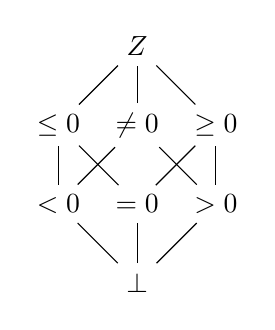
\begin{tikzpicture}
    \node [] (0) at (0, 0) {$\bot$};

    \node [] (1) at (-1, 1) {$< 0$};
    \draw (0) to (1);
    \node [] (2) at (0, 1) {$=0$};
    \draw (0) to (2);
    \node [] (3) at (+1, 1) {$> 0$};
    \draw (0) to (3);
    
    \node [] (4) at (-1, 2) {$\leq 0$};
    \draw (1) to (4);
    \draw (2) to (4);
    \node [] (5) at (0, 2) {$\neq 0$};
    \draw (1) to (5);
    \draw (3) to (5);
    \node [] (6) at (+1, 2) {$\geq 0$};
    \draw (2) to (6);
    \draw (3) to (6);
    
    \node [] (7) at (0, 3) {$\mathbb{Z}$};
    \draw (6) to (7);
    \draw (5) to (7);
    \draw (4) to (7);
  \end{tikzpicture}
  \end{center}

  Then, there is a Galois insertion from $Sign$ to $\pow{\mathbb{Z}}$ defined as:
  $$\gamma(A) = \begin{cases}
    \{ x \mid x \;op\; 0 \} & \text{if } A = op\;0 \\
    \mathbb{Z}              & \text{if } A = \mathbb{Z} \\
    \emptyset & \text{otherwise}
  \end{cases}$$
  $$\alpha(C) = \begin{cases}
    \bot & \text{if } C = \emptyset \\
    op \; 0 & \text{if } C \subseteq \{ x \mid x \; op \; 0 \}
        \mand op \in \{<, >, =, \leq, \geq, \neq \} \\
    \mathbb{Z} & \text{otherwise}
  \end{cases}$$
\end{example}

The fundamental goal of abstract interpretation is to provide an approximation 
of the non-computable aspects of program semantics. The core concept is captured 
by the definition of soundness:

\begin{definition}[Soundness]
  Given an abstract domain $A$, an abstract function $f^\# : A \to A$ is a 
  sound approximation of a concrete function $f : \pow{\states} \to 
  \pow{\states}$ if
  $$\alpha(f(P)) \leq f^\#(\alpha(P))$$
\end{definition}

Hence, the goal of abstract interpretation is to construct a sound 
over-approximation of the program semantics that is computable (efficiently).

\begin{example}
  We can use the sign domain to construct a sound approximation of the
  multiplication operation: 
  \begin{table}[h!]
    \centering
    \begin{tabular}{|c|c|c|c|c|c|c|c|c|}
      \hline
      $\times^\#$ & $\bot$ & $< 0$ & $> 0$ & $= 0$ & $\le 0$ & $\ne 0$ & $\ge 0$ 
                  & $\mathbb{Z}$ \\
      \hline
      $\bot$ & $\bot$ & $\bot$ & $\bot$ & $\bot$ & $\bot$ & $\bot$ & $\bot$ 
             & $\bot$ \\
      \hline
      $< 0$ & $\bot$ & $> 0$ & $< 0$ & $= 0$ & $< 0$ & $\ne 0$ & $\le 0$ 
            & $\mathbb{Z}$ \\
      \hline
      $> 0$ & $\bot$ & $< 0$ & $> 0$ & $= 0$ & $\le 0$ & $\ne 0$ & $\ge 0$ 
            & $\mathbb{Z}$ \\
      \hline
      $= 0$ & $\bot$ & $= 0$ & $= 0$ & $= 0$ & $= 0$ & $= 0$ & $= 0$ & $= 0$ \\
      \hline
      $\le 0$ & $\bot$ & $< 0$ & $\le 0$ & $= 0$ & $\le 0$ & $\ne 0$ & $\le 0$ 
              & $\mathbb{Z}$ \\
      \hline
      $\ne 0$ & $\bot$ & $\ne 0$ & $\ne 0$ & $= 0$ & $\ne 0$ & $\ne 0$ 
              & $\ne 0$ & $\mathbb{Z}$ \\
      \hline
      $\ge 0$ & $\bot$ & $\le 0$ & $\ge 0$ & $= 0$ & $\le 0$ & $\ne 0$ 
              & $\ge 0$ & $\mathbb{Z}$ \\
      \hline
      $\mathbb{Z}$ & $\bot$ & $\mathbb{Z}$ & $\mathbb{Z}$ & $= 0$ 
                   & $\mathbb{Z}$ & $\mathbb{Z}$ & $\mathbb{Z}$ & $\mathbb{Z}$ \\
      \hline
    \end{tabular}
    \caption{Multiplication table for $Sign$ domain}
  \end{table}
\end{example}
